%!TEX program = lualatex
%\documentclass[aspectratio=169,compre%ss,9pt]{beamer}
\documentclass[compress,9pt,xcolor={dvipsnames,table}]{beamer}
\usepackage[T1]{fontenc}
%\usepackage{lmodern}
\usepackage{textcomp}
\usepackage{algorithm}
\usepackage{algorithmic}
\usepackage{tcolorbox}
\usepackage{fontspec}

\usepackage{polyglossia}
\setmainlanguage{english}
\usepackage{tabularx,ragged2e}
\usepackage{booktabs}
\usepackage{dtklogos}
\usepackage{arydshln}
\usepackage{chngpage}

\usepackage{booktabs}
\usepackage{tikz}
\def\checkmark{\tikz\fill[scale=0.4](0,.35) -- (.25,0) -- (1,.7) -- (.25,.15) -- cycle;}
\usepackage{array}
\newcolumntype{L}[1]{>{\raggedright\let\newline\\\arraybackslash\hspace{0pt}}m{#1}}
\newcolumntype{C}[1]{>{\centering\let\newline\\\arraybackslash\hspace{0pt}}m{#1}}
\newcolumntype{R}[1]{>{\raggedleft\let\newline\\\arraybackslash\hspace{0pt}}m{#1}}

\usepackage{multicol}
\usepackage[caption=false]{subfig}
\hypersetup{%
  colorlinks = true,
  linkcolor  = PineGreen!100!black
}

\usepackage{natbib}

\setbeamertemplate{itemize item}{\color{PineGreen}$\bullet$}
\setbeamertemplate{itemize subitem}{\color{PineGreen!25}$\circ$}
\setbeamercolor{enumerate item}{fg=PineGreen}
\setbeamercolor{caption name}{fg=PineGreen}

\setmainfont[]{Cardo} % sets the roman font
%\setsansfont[]{Alegreya} % sets the sans font % Vallkorn, Alegreya
\setsansfont[]{PT Sans} % sets the sans font
\setmonofont[]{Consolas} % sets the monospace font
\setbeamertemplate{navigation symbols}{}
    \expandafter\def\expandafter\insertshorttitle\expandafter{%
      \insertshorttitle\hfill%
      \insertframenumber\,/\,\inserttotalframenumber}

\usetheme{Szeged}
\usecolortheme{spruce}

\title[Smart usage of context information for the analysis, design and generation of power-aware polices for mobile sensing apps]{ Smart usage of context information for the analysis, design and generation of power-aware polices for mobile sensing apps}
\author[Rafael Perez Torres]{Presented by: Rafael Perez Torres\\[0.5cm] Thesis advisors:\\PhD Cesar Torres Huitzil\\PhD Hiram Galeana Zapien}
\institute{LTI Cinvestav Tamaulipas}
%\date{\today}
\date{}

\begin{document}
\begin{frame}[plain]
  % {
  % \begin{center}
  % 
\includegraphics[scale=0.12]{../../../resources/images/vectors/cinvestav-logo-no-text}
  % \end{center}
  % }
  \begin{center}
  
\includegraphics[scale=0.12]{../../../resources/images/vectors/cinvestav-logo-no-text}
  \end{center}
  \titlepage
  
\end{frame}

%\frame{\maketitle}

\begin{frame}{Table of contents}
	\tableofcontents[hideallsubsections]
\end{frame}

\section{Problem statement}
\subsection{Problem statement}

\begin{frame}[t]\frametitle{Introduction}
\begin{itemize}
  \item The popularity of mobile devices is a result of advances in their computation, sensing, and communication dimensions~\cite{Islam2014}.
  % \item Possibility of installing new mobile applications.
  \item Smartphone's sensing facilities improve interaction with user, turning them into \emph{omni-sensors} able to \emph{know} about its surrounding environment.
  % \item Hence, mobile devices have achieved a considerable degree of sensitivity that tries to mimic the sense of humans.
  \item Mobile devices have become \emph{context-aware}, gaining understanding about user's activity and environment.
  % \item \emph{Context} refers to a four-dimensional space composed of \emph{computing context}, \emph{physical context}, \emph{time context}, and \emph{user context}~\cite{Chen2000}.
  \item However, battery is not evolving at the same pace than the advances in other smartphone's characteristics~\cite{Kjaergaard2012}, growing only 5\% each year~\cite{Ma2012}.
  \item The energy constraint becomes more critical when continuous access to sensors is needed, which is the core requirement of \textbf{mobile sensing applications}.
\end{itemize}
\end{frame}

\begin{frame}[t]\frametitle{Problem antecedents: Stages of mobile sensing applications}
\begin{figure}[tb]
  \centering
  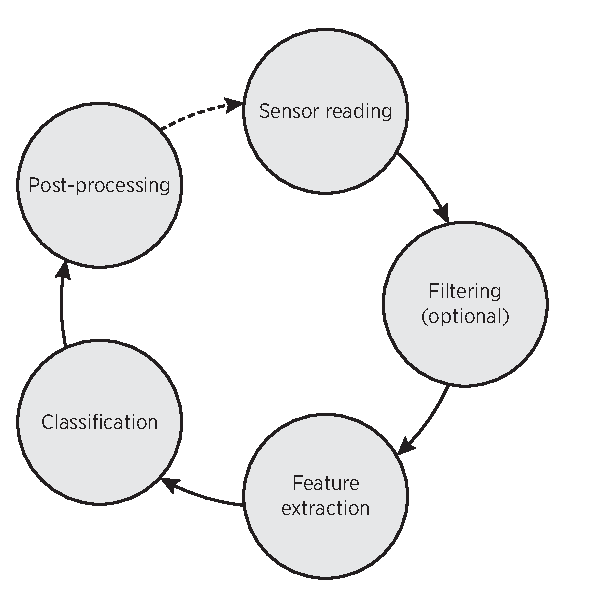
\includegraphics[width=\textwidth]{../../../resources/images/vectors/msa-stages}
  \caption{Stages of mobile sensing applications}
  \label{fig:msa-stages}
\end{figure}
There is a tradeoff between the accuracy of context information retrieved and the associated energy consumption~\cite{Sim2014,Rachuri2012}.
How to face it?
\end{frame}

\begin{frame}\frametitle{Hypothesis}
\begin{tcolorbox}[title=Hypothesis,colframe=PineGreen]
Intelligent policies produced through context information built from sensors data can be employed to reduce the energy consumption in a mobile device when performing continuous sensor readings.
\end{tcolorbox}

{
\small
\begin{itemize}
  \item An intelligent policy is a special rule that defines how sensors should be accessed in order to reduce the energy consumption and achieve the requirements of a mobile app.
  It is intelligent in terms of self-adaptness to changes detected in context information.
  \item This research work is aimed at employing GPS and inertial sensors data (accelerometer) for inferring context information in terms of mobility patterns.
  This context information will then be exploited to adapt sensors' operation and produce power savings.
\end{itemize}
}
\end{frame}

\begin{frame}\frametitle{Problem statement}
\begin{tcolorbox}[title=Problem statement: Mobility pattern identification,colframe=PineGreen]
\small
Given a set $V = \left\{v_{1}, v_{2}, \dotsc, v_{n}\right\}$ of data values read from sensor $S$ in the time interval $T  \in [t_{1}, t_{2}]$, identify the current mobility pattern $p_{S}$ that represents the activity of user.

\begin{equation}
  \text{PatternIdentifier}( V ) \longrightarrow{} p_{S} \in Patterns
\end{equation}

Where $Patterns$ is a set of patterns that represent an interesting state in user mobility, specifically the set $\left\{no\_movement, walking, running, vehicle\_transportation\right\}$.

\begin{figure}[tb]
  \centering
  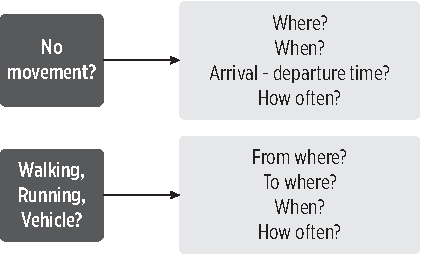
\includegraphics[scale=0.5]{../../../resources/images/vectors/mobility-patterns-implications}
  \caption{Context information related to mobility patterns}
  \label{fig:mobility-patterns-implications}
\end{figure}

\end{tcolorbox}




\end{frame}

\begin{frame}\frametitle{Problem statement}
\begin{tcolorbox}[title=Problem statement: Policy generation,colframe=PineGreen]
\small
Given the set of detected mobility patterns $\mathcal{P} = \{ p_{S_1}, p_{S_2}, \ldots, p_{S_n} \}$ in data from sensors $\mathcal{S} = \{ S_1,S_2,\ldots, S_n \}$, parameters for assigning weight to energy $e$ and accuracy $a$, and physical constraints status $c$ of a mobile device, find a policy that select the proper set of sensors $\mathcal{S}_{new}$ and its associated configuration $\mathcal{S}_{new_{conf}}$  while meeting application requirements.

\begin{equation}
  \text{PolicyGeneration}( \mathcal{P}_{\mathcal{S}}, e, a, c ) \longrightarrow{} \mathcal{S}_{new}, \mathcal{S}_{new_{conf}}
\end{equation}

The $\mathcal{S}_{new_{conf}}$ configuration is referred as the \emph{adaptative duty cycle} of associated sensor.
\end{tcolorbox}
\end{frame}

\begin{frame}\frametitle{Interaction between problems}
\begin{figure}[tb]
  \centering
  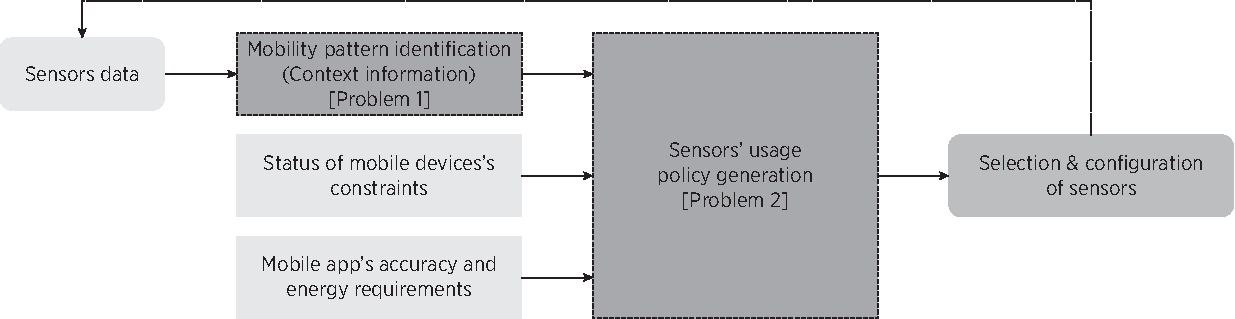
\includegraphics[width=\textwidth]{../../../resources/images/vectors/problems-incorporation}
  \caption{Interaction between the thesis work's problems}
  \label{fig:probems-incorporation}
\end{figure}
\end{frame}

\begin{frame}[t]\frametitle{Problem's scenario}
\begin{figure}[tb]
  \centering
  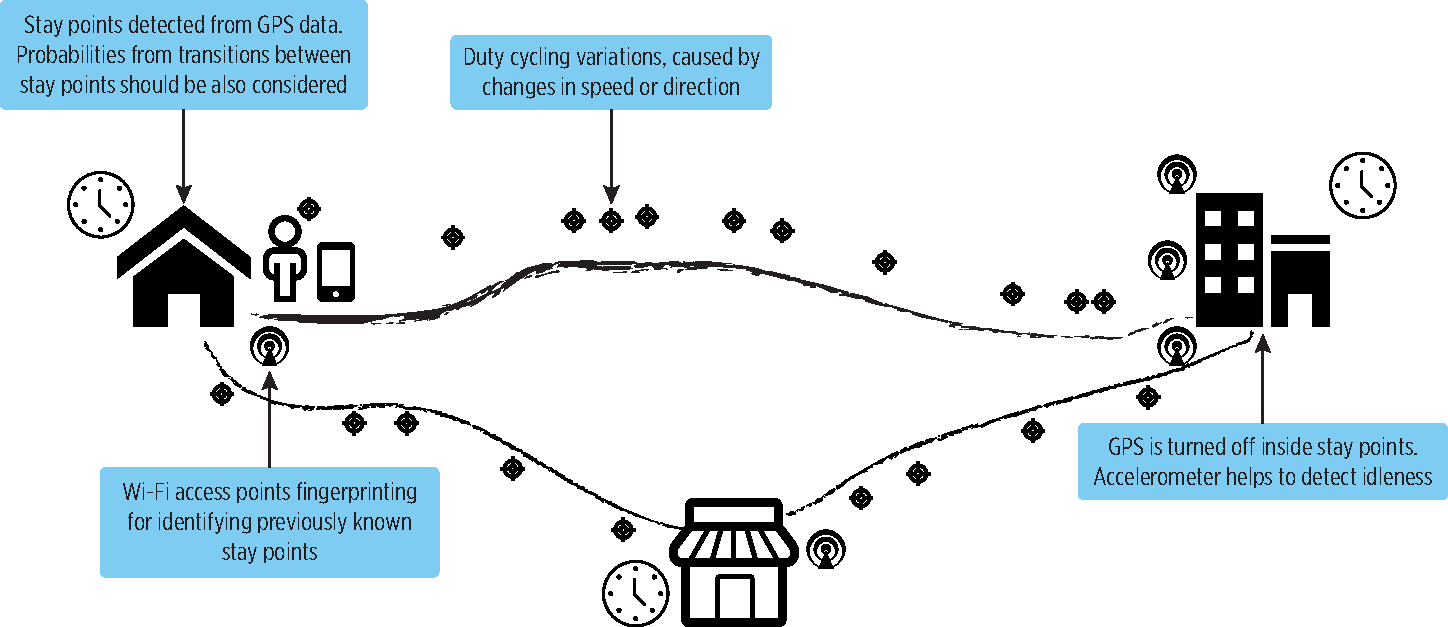
\includegraphics[width=\textwidth]{../../../resources/images/vectors/scenario}
  \caption{Basic problem's scenario}
  \label{fig:scenario}
\end{figure}
\end{frame}


\section{Methodology}
\subsection{Methodology}
\begin{frame}\frametitle{Methodology}
\begin{enumerate}
  \item \textbf{Familiarization with state-of-art power-aware sensing related techniques}
  \item \textbf{Formal definition and selection of mobility patterns to be identified}
  \item \textbf{Research on pattern recognition algorithms focused on mobility patterns identification}
  \item \textbf{Design of the Pattern Identification Element (PIE)}
  \item Research on and proposition of adaptive policies for energy efficient usage of sensors
  \item Design of the Policy Generation Element (PGE)
  \item Development of a middleware involving the PIE and PGE for the Android platform
  \item Experimentation in terms of accuracy and energy efficiency
\end{enumerate}
\end{frame}


\section[State-of-art]{State of art related techniques}
\subsection{State of art}

\begin{frame}\frametitle{The smartphone as a three-dimensional device}
\begin{figure}[tb]
  \centering
  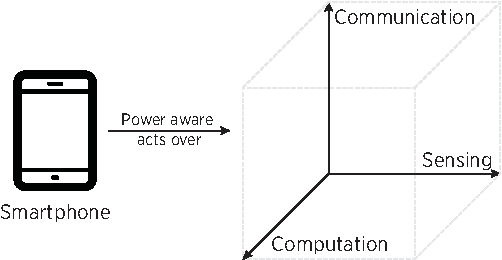
\includegraphics[width=0.75\textwidth]{../../../resources/images/vectors/smartphone-dimensions}
  \caption{The smartphone as a three-dimensional device}
  \label{fig:smartphone-three-dimensional}
\end{figure}
\end{frame}


\begin{frame}\frametitle{Taxonomy of state of art solutions}
\begin{figure}[tb]
  \centering
  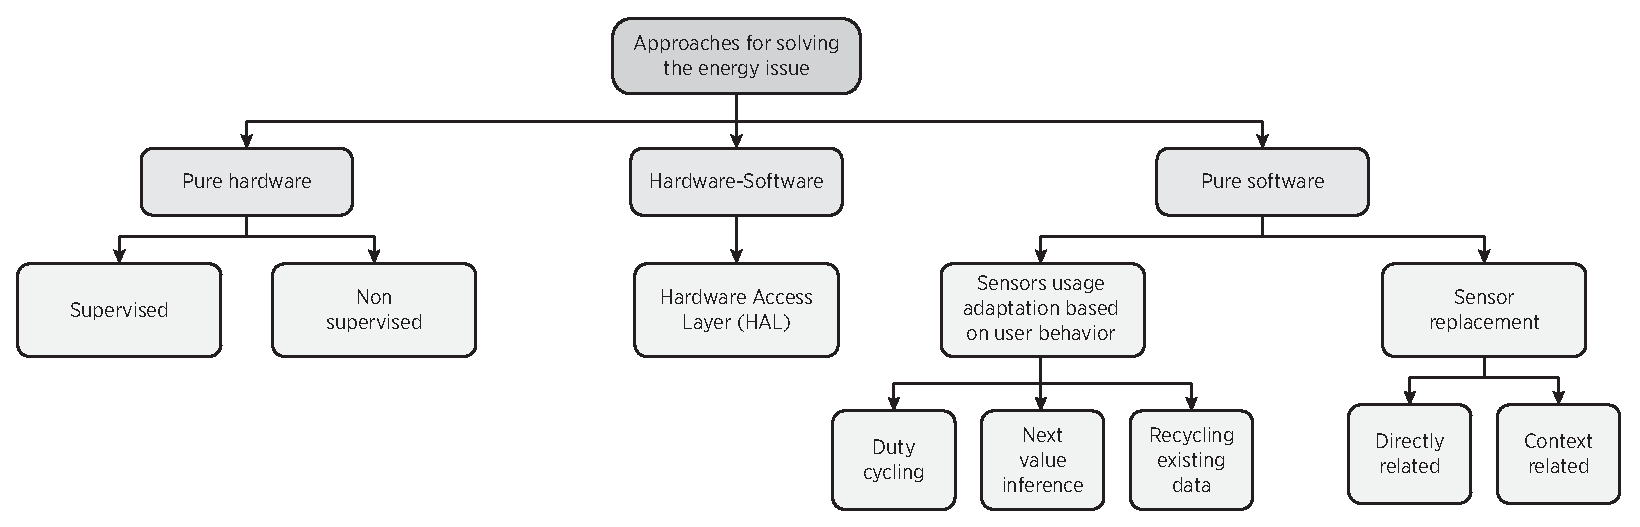
\includegraphics[width=\textwidth]{../../../resources/images/vectors/approaches-taxonomy}
  \caption{Taxonomy of solutions, seen from the sensors adaptation's perspective}
  \label{fig:taxonomy}
\end{figure}
\end{frame}

\begin{frame}\frametitle{Distribution of approaches}
\begin{figure}[tb]
  \centering
  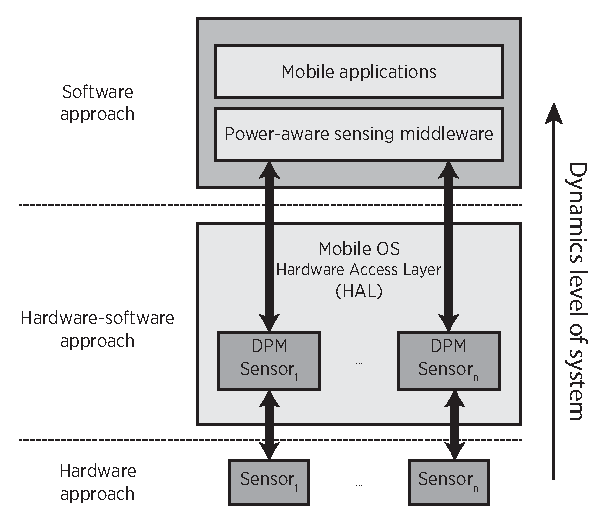
\includegraphics[scale=0.72]{../../../resources/images/vectors/approaches-distribution}
  \caption{Distribution of approaches across mobile platform's layers}
  \label{fig:distribution}
\end{figure}
\end{frame}


\begin{frame}[t]\frametitle{Characteristics of pure software approach solutions}
\begin{tcolorbox}[title=Distinctive characteristics of pure software solutions,colframe=PineGreen]
\small
\begin{itemize}
  \item \textbf{Optimization oriented (OO)}: Works can follow an optimization orientation focused on minimizing energy consumption and/or the error in activity tracking.
  \item \textbf{Online learning (OL)}: Solutions can incorporate mechanisms for online learning (OL) from context information, enabling predictive features thanks to observance over long-time windows of sensory data.
  \item \textbf{User state oriented (US)}: Solutions can employ an enriched version of the context information, known as user state (US) for allowing the device to become fully activity-aware and ease its adaptation over the sensing dimension.
\end{itemize}
\end{tcolorbox}
\end{frame}

\begin{frame}[t]\frametitle{Framework for analyzing pure software solutions}
\begin{tcolorbox}[title=Framework for analyzing pure software solutions,colframe=PineGreen]
\small
Granularity of context information
\begin{itemize}
  \item Input data type
  \item Classifier or machine learning technique
  \item Length of time window
\end{itemize}
\end{tcolorbox}
\end{frame}


\begin{frame}[t]\frametitle{Framework for analyzing pure software solutions}
\begin{figure}[tb]
  \centering
  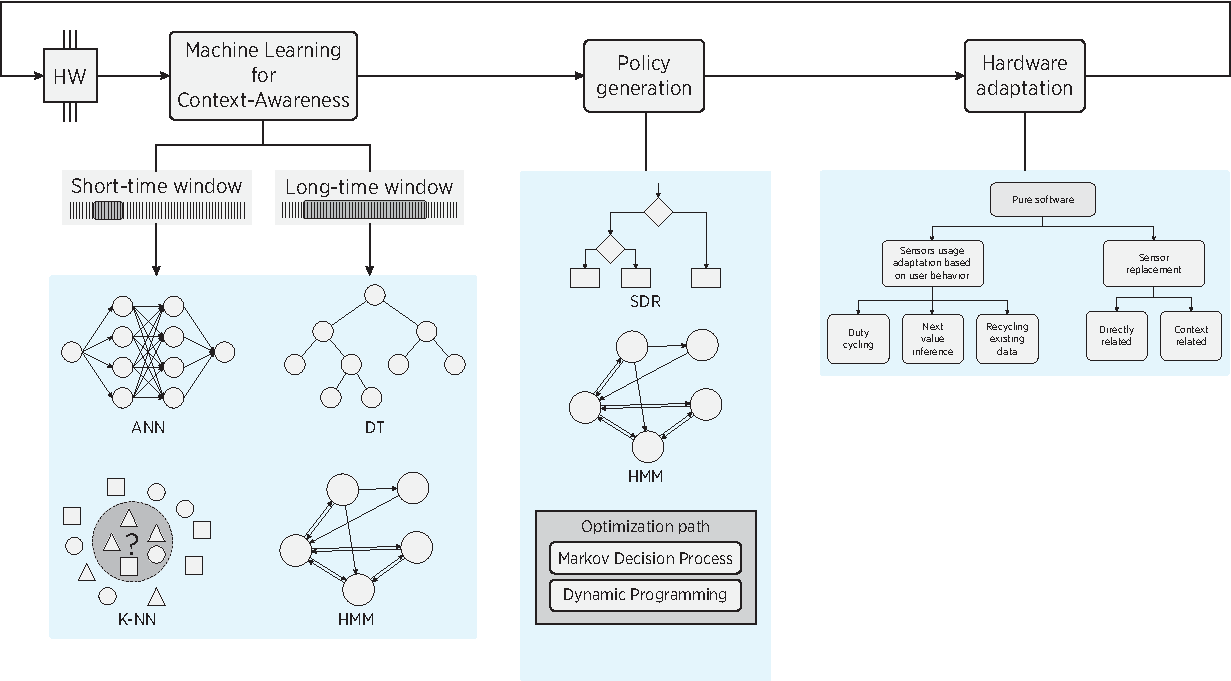
\includegraphics[width=\textwidth]{../../../resources/images/vectors/dual-taxonomy}
  \caption{Decomposition of solutions}
  \label{fig:dual-taxonomy}
  \end{figure}
\end{frame}


\begin{frame}[t]\frametitle{State-of-art solutions}
\begin{table}
    \centering
    \scriptsize{}
    \resizebox{\textwidth}{!} { 
    \begin{tabular}{C{0.11\textwidth}C{0.2\textwidth}C{0.17\textwidth}C{0.15\textwidth}C{0.09\textwidth}C{0.05\textwidth}C{0.05\textwidth}C{0.05\textwidth}}
    % \begin{tabular}{C{0.15\textwidth}C{0.22\textwidth}C{0.25\textwidth}C{0.27\textwidth}}
    \toprule
    \textbf{Name} & \textbf{Variants} & \textbf{Machine learning technique} & \textbf{Sensors involved} & \textbf{Complexity} & \textbf{OL} & \textbf{OO} & \textbf{US} \\
    \midrule

    
    % Category Basic context policy (short time window)
    \emph{G-Sense}      \cite{Perez2010} & User behavior learning (DC) & SDR & GPS & low \\

    \cmidrule(l){1-8}
    Perez-Torres           \cite{Perez-Torres2012} & User behavior learning (DC) & SDR & GPS & low \\

    \cmidrule(l){1-8}
    \emph{SenseLess}    \cite{Abdesslem2009} & User behavior learning (DC), Sensor replacement (CR, DR) & SDR & WPS, GPS, ACC & low \\
    
    \cmidrule(l){1-8}
    \emph{SensTrack}    \cite{Zhang2013} & User behavior learning (DC), Sensor replacement (CR, DR) & SDR & ACC, orientation sensor, GPS, WPS & low \\
    % \emph{SensTrack}    \cite{Zhang2013} & User behavior learning (DC), Sensor replacement (CR,DR) & SDR, Gaussian Regression Model (GRM) & ACC, orientation sensor, GPS, WPS & low \\
    
    \cmidrule(l){1-8}
    Man and Ngai           \cite{Man2014} & User behavior learning (DC, VI), Sensor replacement (CR) & SDR & ACC, magnetic field sensor, GPS & low \\
    % Not given           \cite{Man2014} & User behavior learning (DC), Sensor replacement (CR) & SDR (Trigonometrical approach) & ACC, magnetic field sensor, GPS & low \\

    \cmidrule(l){1-8}
    \emph{EnLoc}        \cite{Constandache2009} & User behavior learning (DC, VI), Sensor replacement (DR) & SDR, Mobility Tree & WPS, GPS, cellular ID & medium & & \checkmark \\
    
    \cmidrule(l){1-8}
    \emph{EnTracked}    \cite{Kjaergaard2009} & User behavior learning (DC), Sensor replacement (CR) & SDR & ACC, GPS & medium & & \checkmark \\
    \bottomrule
    \end{tabular}
    }
    \protect\caption{Pure software solutions. (OL: Online Learning from user data, OO: Optimization Oriented solution, US: User State context insight)\label{tab:works-software-approach-1}}
\end{table}
\end{frame}

\begin{frame}[t]\frametitle{State-of-art solutions}
\begin{table}
    \centering
    \scriptsize{}
    \resizebox{\textwidth}{!} { 
    \begin{tabular}{C{0.11\textwidth}C{0.2\textwidth}C{0.17\textwidth}C{0.15\textwidth}C{0.09\textwidth}C{0.05\textwidth}C{0.05\textwidth}C{0.05\textwidth}}
    % \begin{tabular}{C{0.15\textwidth}C{0.22\textwidth}C{0.25\textwidth}C{0.27\textwidth}}
    \toprule
    \textbf{Name} & \textbf{Variants} & \textbf{Machine learning technique} & \textbf{Sensors involved} & \textbf{Complexity} & \textbf{OL} & \textbf{OO} & \textbf{US} \\
    \midrule

    % Category Medium context-aware policy
    % Not given           \cite{AlvarezDeLaConcepcion2014,Morillo2015} & --- & Ameva algorithm, majority vote system & ACC & low \\
    Alvarez, Morillo           \cite{AlvarezDeLaConcepcion2014,Morillo2015} & --- & Ameva algorithm & ACC & medium \\
    
    \cmidrule(l){1-8}
    Mazilu           \cite{Mazilu2013} & Sensor replacement (CR) & DT & Temperature, humidity, pressure & medium \\
    % Not given           \cite{Mazilu2013} & Sensor replacement (CR) & DT (C4.5) & Temperature, humidity, pressure & medium \\

    \cmidrule(l){1-8}
    Srinivasan           \cite{Srinivasan2012} & User behavior learning (DC) & DT & ACC & medium \\
    
    \cmidrule(l){1-8}
    Khalifa           \cite{Khalifa2015} & Sensor replacement (CR) & KNN & Model of ACC-based harvesting device & medium \\
    % Not given           \cite{Khalifa2015} & Sensor replacement (CR) & KNN & Model of ACC-based harvesting device & low \\
    \bottomrule
    \end{tabular}
    }
    \protect\caption{Pure software solutions. (OL: Online Learning from user data, OO: Optimization Oriented solution, US: User State context insight)\label{tab:works-software-approach-2}}
\end{table}
\end{frame}


\begin{frame}[t]\frametitle{State-of-art solutions}
\begin{table}
    \centering
    \scriptsize{}
    \resizebox{\textwidth}{!} { 
    \begin{tabular}{C{0.11\textwidth}C{0.2\textwidth}C{0.17\textwidth}C{0.15\textwidth}C{0.09\textwidth}C{0.05\textwidth}C{0.05\textwidth}C{0.05\textwidth}}
    % \begin{tabular}{C{0.15\textwidth}C{0.22\textwidth}C{0.25\textwidth}C{0.27\textwidth}}
    \toprule
    \textbf{Name} & \textbf{Variants} & \textbf{Machine learning technique} & \textbf{Sensors involved} & \textbf{Complexity} & \textbf{OL} & \textbf{OO} & \textbf{US} \\
    \midrule

    % Category Long time window
    \emph{SensLoc}         \cite{Kim2010} & User behavior learning (DC, RD), Sensor replacement (CR) & SDR & Wi-Fi fingerprinting, GPS, ACC & medium & \checkmark & \\
    % \emph{SensLoc}         \cite{Kim2010} & User behavior learning (DC), Sensor replacement (CR,DR) & SDR (Tanimoto coefficient and ACC variance) & Wi-Fi fingerprinting, GPS, ACC & medium & \checkmark & & \checkmark \\
    
    \cmidrule(l){1-8}
    \emph{CAPS}         \cite{Paek2011} & User behavior learning (DC, RD), Sensor replacement (CR) & SDR & GPS, cellular ID & medium & \checkmark \\
    % SDR (Smith-Waterman algorithm) CR because location is processed alternatively with this algorithm

    \cmidrule(l){1-8}
    \emph{RAPS}         \cite{Paek2010} & User behavior learning (DC, RD), Sensor replacement (CR, DR) & SDR & WPS, GPS, ACC, Bluetooth, cellular ID & medium & \checkmark \\
    
    % In-between Category Optimization + long time window
    \cmidrule(l){1-8}
    \emph{A-Loc}        \cite{Lin2010} & User behavior learning (DC, RD), Sensor replacement (CR, DR) & HMM, Bayesian estimation framework & GPS, WPS, Bluetooth, cellular ID & medium & \checkmark & \checkmark  \\
    
    \cmidrule(l){1-8}
    \emph{SmartDC}      \cite{Chon2011} & User behavior learning (DC, RD), Sensor replacement (CR, DR) & HMM and LZ predictor & GPS, WPS, Wi-Fi and cellular ID fingerprinting & medium & \checkmark & \checkmark \\
    
    \bottomrule
    \end{tabular}
    }
    \protect\caption{Pure software solutions. (OL: Online Learning from user data, OO: Optimization Oriented solution, US: User State context insight)\label{tab:works-software-approach-3}}
\end{table}
\end{frame}

\begin{frame}[t]\frametitle{State-of-art solutions}
\begin{table}
    \centering
    \scriptsize{}
    \resizebox{\textwidth}{!} { 
    \begin{tabular}{C{0.11\textwidth}C{0.2\textwidth}C{0.17\textwidth}C{0.15\textwidth}C{0.09\textwidth}C{0.05\textwidth}C{0.05\textwidth}C{0.05\textwidth}}
    % \begin{tabular}{C{0.15\textwidth}C{0.22\textwidth}C{0.25\textwidth}C{0.27\textwidth}}
    \toprule
    \textbf{Name} & \textbf{Variants} & \textbf{Machine learning technique} & \textbf{Sensors involved} & \textbf{Complexity} & \textbf{OL} & \textbf{OO} & \textbf{US} \\
    \midrule

    % Category Full context-aware policy
    \emph{Jigsaw}       \cite{Lu2010} & User behavior learning (DC), Sensor replacement (CR) & Microphone: NB with Gaussian Mixture Model (GMM). ACC: DT. GPS: MDP. & ACC, Microphone, GPS & high & & \checkmark & \checkmark \\
    
    \cmidrule(l){1-8}
    Donohoo           \cite{Donohoo2014} & User behavior learning (DC) & Several. KNN and NN selected as best. & ACC, GPS, WPS, cellular ID, light, device data, mobile app requirements & high & & & \checkmark \\

    \cmidrule(l){1-8}
    \emph{EEMSS}        \cite{Wang2009} & User behavior learning (DC), Sensor replacement (CR, DR) & GPS and ACC: SDR. \newline Microphone: SSCH algorithm. & ACC, microphone, GPS & high & & & \checkmark \\

    \cmidrule(l){1-8}
    \emph{iLoc}         \cite{MaY2009} & User behavior learning (RD), Sensor replacement (CR) & HMM & Wi-Fi \& GSM fingerprinting & high & \checkmark & & \checkmark  \\
    
    \cmidrule(l){1-8}
    Yurur           \cite{Yurur2014} & User behavior learning (DC, RD) & HMM & ACC & high & \checkmark & & \checkmark \\
    
    \cmidrule(l){1-8}
    \emph{FreeTrack}    \cite{Chon2014} & User behavior learning (DC, RD), Sensor replacement (CR, DR) & HMM & GPS, Wi-Fi, cellular ID, battery status & high & \checkmark & & \checkmark \\
    
    \bottomrule
    \end{tabular}
    }
    \protect\caption{Pure software solutions. (OL: Online Learning from user data, OO: Optimization Oriented solution, US: User State context insight)\label{tab:works-software-approach-4}}
\end{table}
\end{frame}




\section{Proposed solution}
\subsection{Proposed solution}
\begin{frame}[t]\frametitle{Proposed solution}
\begin{figure}[tb]
  \centering
  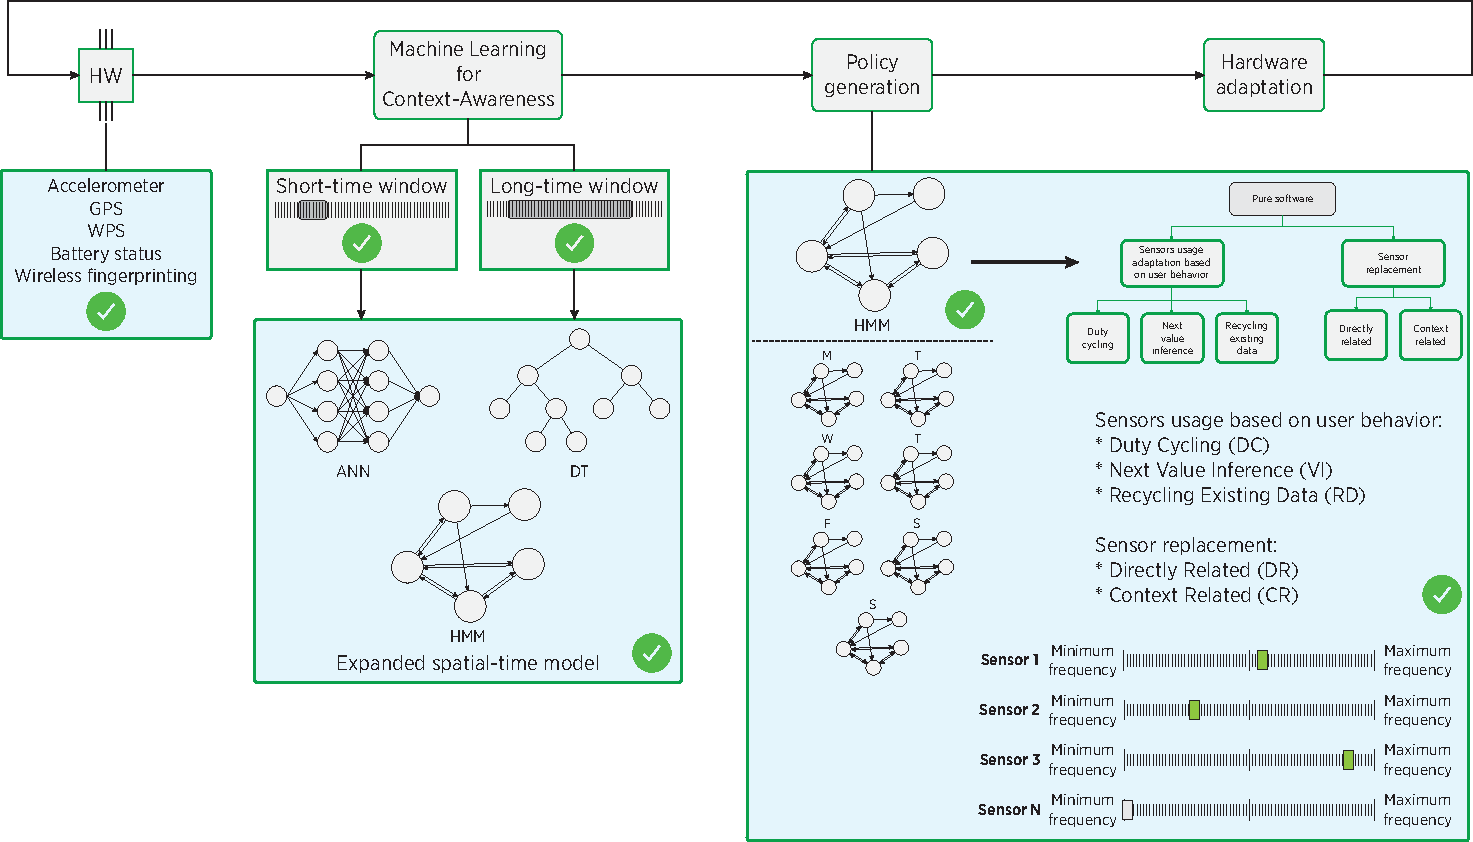
\includegraphics[width=\textwidth]{../../../resources/images/vectors/dual-taxonomy-ours}
  \caption{Decomposition of our solution}
  \label{fig:dual-taxonomy-ours}
  \end{figure}
% At the end we can describe that:
% \begin{itemize}
  % \item In the ML block, we are going to produce an enhanced-expanded spatial-time model by:
  % \begin{itemize}
  %   \item Classifying accelerometer data in user activity.
  %   \item Obtaining context information from other sources:
  %   \begin{itemize}
  %     \item Fingerprinting, battery status.
  %   \end{itemize}
  %   \item Obtaining speed from GPS
  %   \item Obtaining location from GPS and WPS
  % \end{itemize}
  % \item In the policy block, we will try to adapt the sensing dimension spliting the problem into:
  % \begin{itemize}
  %   \item Learning and detection of stay points (Already covered)
  %   \item Learning and detection (tracking) of trajectories.
  % \end{itemize}
  % \item In the HW adaptation bloc, we will use several variants of the PS approach.
  % For instance, we will do:
  % \begin{itemize}
  %   \item Sensor replacement, Context related (battery) and Direct related (WPS).
  %   \item Adapt accordingly to what is learned from user through Duty Cycling (DC) and Recycling existing Data (RD).
  %   Maybe we will use Next Value Inference (VI) in the policy, when we adapt under uncertainty.
  %   For instance, we are 80\% sure that user is running, we will proceed with caution adapting duty cycle with fine granularity, this is negotiable.
  % \end{itemize}
  % \item At the end, we are trying to maintain sensors within a range that allows to perform the tracking but considering the trade-off.
% \end{itemize}
\end{frame}

\begin{frame}[t]\frametitle{Proposed solution}
\begin{figure}[tb]
  \centering
  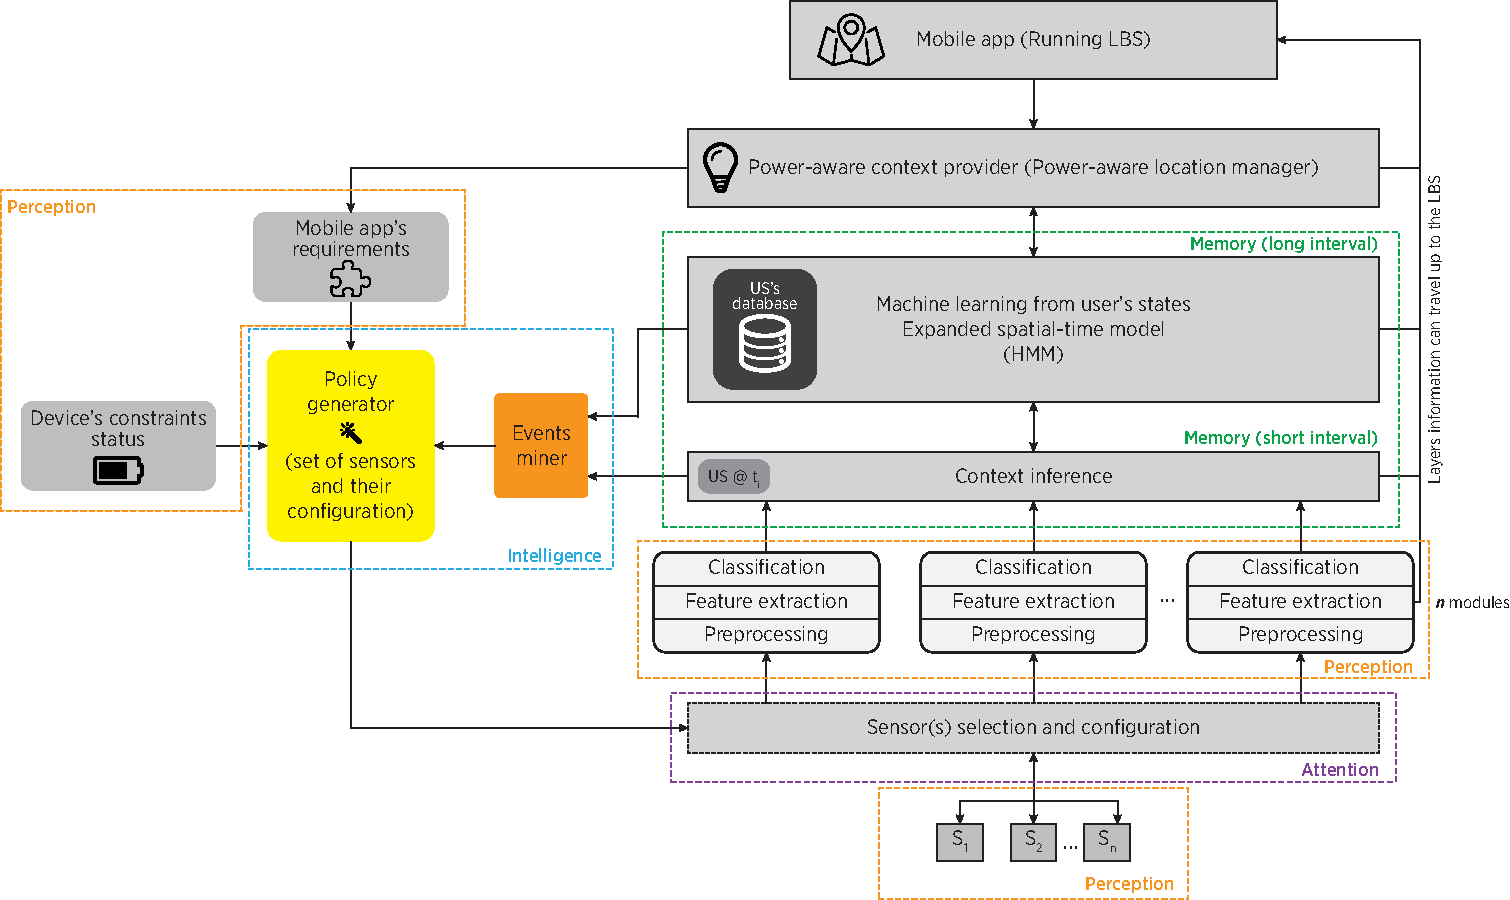
\includegraphics[width=0.9\textwidth]{../../../resources/images/vectors/solution-general-overview}
  \caption{Overview of current solution}
  \label{fig:solution}
\end{figure}
\end{frame}

\begin{frame}[t]\frametitle{The model of information learned in proposed solution}
\begin{figure}[tb]
  \centering
  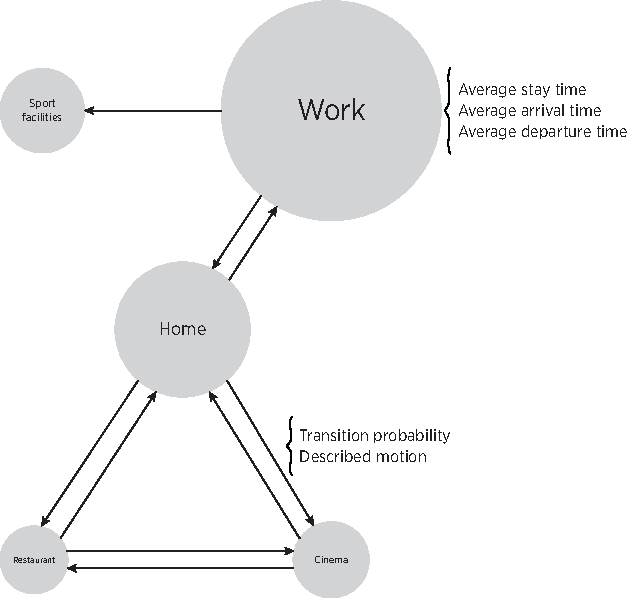
\includegraphics[scale=0.6]{../../../resources/images/vectors/mobility-graph}
  \caption{Basic unit of information learned (User state)}
  \label{fig:basic-unit-of-information-learned}
\end{figure}
\end{frame}

\begin{frame}[t]\frametitle{The model of information learned in proposed solution}
\begin{figure}[tb]
  \centering
  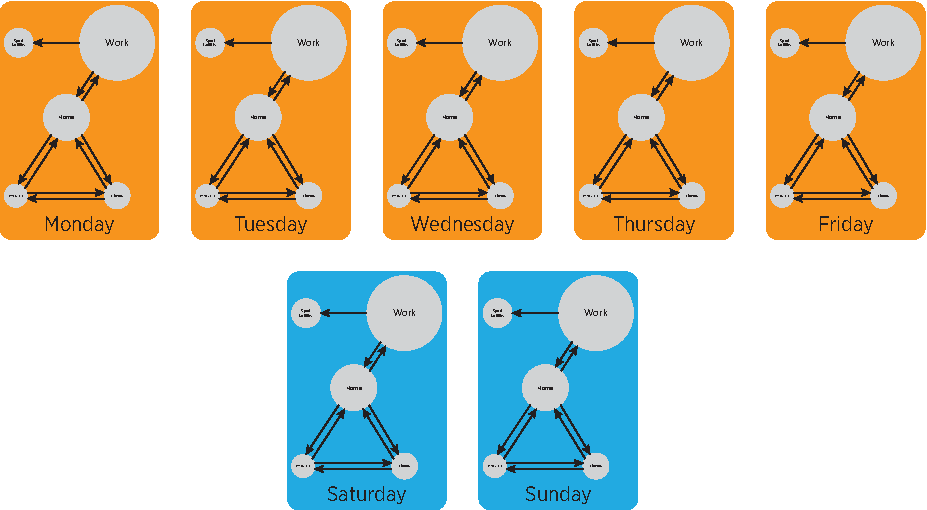
\includegraphics[width=\textwidth]{../../../resources/images/vectors/mobility-graph-larger-time-window-two-rows}
  \caption{Mobility patterns learned over longer time windows}
  \label{fig:information-learned-longer-time-windows}
\end{figure}
\end{frame}


\section{Important results}
\subsection{Important results}
\label{sub:important_results}
\begin{frame}[t]\frametitle{Results of early experimentation}
\begin{itemize}
  \item The feasibility of on-device detection of stay points has been partially prooved through experimentation.
  \item These experiments ensure proper calculations of stay points, even under mobile device constraints.
  \item A slight adaptation of classic algorithms for stay points detection has been implemented.
  \item Such variant (sigma) obeys an event-oriented paradigm, which is a trend for \textbf{proactive} long-term applications focused on learning patterns from user activity.
\end{itemize}
\end{frame}

\begin{frame}[t]\frametitle{On-device stay points detection platform}
    
\begin{figure}[tb]
  \centering
  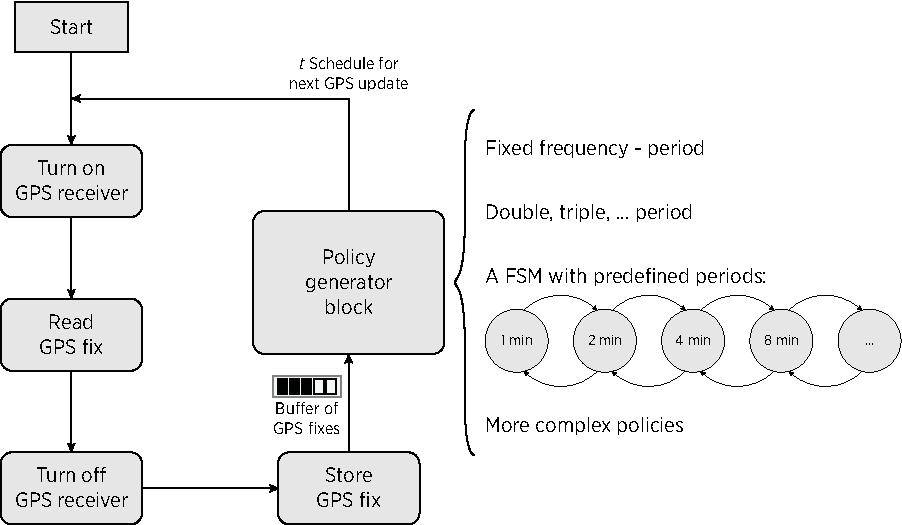
\includegraphics[scale=0.5]{../../../resources/images/vectors/policy-creator-methodology}
  \caption{Logical workflow of the platform for on-device stay points detection}
  \label{fig:logical-workflow}
\end{figure}

\end{frame}

\begin{frame}[t]\frametitle{Results of early experimentation}
\begin{itemize}
  \item The first experiment is aimed at ensuring te calculation of stay points locally at the smartphone (Samsung Galaxy Note II, Quadcore 1.6 GHz processor, 16 GB RAM, 3,100 mAh battery).
  \item Both versions of the algorithm for stay points detection, original (buffered) and sigma, have been employed.  
\end{itemize}
\end{frame}


\begin{frame}[t]\frametitle{Results of early experimentation}
\begin{itemize}
  \item Policies implemented:
  \begin{itemize}
  \item Periodic GPS sampling: 1, 3, and 5 minutes.
  \item FSM doubling policy. Starting with 1 minute reading period, doubling if no movement within a threshold of 50 meters was detected (Upper limit 16 minutes).
  \item FSM linear policy. Possible fixed states at 1, 3, 6, 9, 12 and 15 minutes.
  \end{itemize}
  \item The parameters for running the stay point detection algorithms for all tests were set at 10 minutes for $\theta_{tmin}$, 1 hour for $\theta_{tmax}$ and 150 m for $\theta_{d}$.
\end{itemize}
\begin{table}[t]
\small{}
\centering
\resizebox{\textwidth}{!}{%
\begin{tabular}{@{}ccccccc@{}}
\toprule
\textbf{\begin{tabular}[c]{@{}c@{}}GPS reading\\ period\end{tabular}} & \textbf{Algorithm} & \textbf{\begin{tabular}[c]{@{}c@{}}Stay points\\ detected\end{tabular}} & \textbf{Average fixes} & \textbf{Maximum fixes} & \textbf{GPS accesses} & \textbf{Running time (hours)} \\ \midrule

1 minute &  Sigma Montoliou     & 27 & 70 & 652 & 2251 & 43.68 \\
1 minute &  Buffered Montoliou  & 26 & 79 & 685 & 2334 & 43.92 \\
\cmidrule{1-7}

3 minutes & Sigma Montoliou     & 47 & 27 & 248 & 1361 & 71.84 \\
3 minutes & Buffered Montoliou  & 28 & 41 & 248 & 1241 & 64.96 \\
\cmidrule{1-7}

5 minutes & Sigma Montoliou     & 43 & 25 & 154 & 1119 & 95.88 \\
5 minutes & Buffered Montoliou  & 45 & 21 & 154 & 1021 & 87.78 \\
\cmidrule{1-7}

Doubling 1-2-4-8-16 & Sigma Montoliou   & 59 & 17 & 80 & 1223 & 189.69 \\
Linear 1-3-5-9-12-15 &  Sigma Montoliou & 35 & 21 & 84 & 888 & 144.85 \\

\bottomrule
\end{tabular}
}
\caption{Results of the first experiment}
\label{tbl:experiment-1}
\end{table}
\end{frame}


% \section{Scientific publications produced}
\subsection{Publications}
\begin{frame}[t]\frametitle{Scientific products}
\begin{itemize}
  \item As a product of the study and analysis of related solutions, we have prepared a survey covering:
  \begin{itemize}
    \item The characteristics of smartphone-based sensing.
    \item The power-awareness in smartphone-based sensing and related areas.
    \item A taxonomy of the different solutions aimed at energy efficiency in smartphone-based sensing.
    \item A framework for dissecting and studying the characteristics of these solutions.
    \item The different tendencies and open challenges of the field.
  \end{itemize}
  \item The aforementioned experimentation is also under expansion and improvement for preparing an article focused on:
  \begin{itemize}
    \item On-device learning of mobility information following an event-oriented perspective.
    \item The employment of such information for adapting the sensing dimension of smartphone looking for energy efficiency.
    \item Setting the base for further modules and strategies for boosting the learning of mobility patterns.
    \item All of these targetted at building the main blocks of our solution.
  \end{itemize}
\end{itemize}
\end{frame}


\section{Future work}
\subsection{Future work}
\begin{frame}[t]\frametitle{Future work}
    
  \definecolor{colorA}{gray}{0.85}
  \definecolor{colorB}{gray}{0.95}
  \definecolor{colorStep}{gray}{1}
  \definecolor{cyellow1}{RGB}{240,236,43}
  \definecolor{cgreen1}{RGB}{73,237,55}

  \newlength{\longitudCelda}
  \setlength{\longitudCelda}{75mm}

  \begin{table}[!h]
  {
    \scalebox{0.75}{
    \small
      \begin{tabular*}{16.5cm}{lp{\longitudCelda}*{7}{c}}
          & & \multicolumn{1}{ :c: }{\tiny 2014} & \multicolumn{3}{ c: }{\tiny 2015} & \multicolumn{3}{ c: }{\tiny 2016}  \\
          \cline{3-9}

          \multicolumn{2}{c:}{}
          & \multicolumn{1}{c:}{\tiny 3\textsuperscript{rd}} 
          & \tiny 1\textsuperscript{st} & { \tiny 2\textsuperscript{nd}} & \multicolumn{1}{c:}{ \tiny 3\textsuperscript{rd}}
          & \tiny 1\textsuperscript{st} & \tiny 2\textsuperscript{nd} & \multicolumn{1}{c:}{ \tiny 3\textsuperscript{rd}} \\
          \cline{3-9}

          % Step 1
          \rowcolor{colorStep}
          & \multicolumn{1}{c}{\scriptsize \textsc{Step I}}  & & & & & & \\
          
          \rowcolor{colorA}
          1 & \multicolumn{1}{p{\longitudCelda}:}{State-of-art reading} &
          \cellcolor{cgreen1} & \cellcolor{cgreen1} & &
          & & & \\

          \rowcolor{colorB}
          2 & \multicolumn{1}{p{\longitudCelda}:}{State-of-art works categorization} &
          & \cellcolor{cgreen1} & \cellcolor{cgreen1} &
          & & & \\

          \rowcolor{colorA}
          3 & \multicolumn{1}{p{\longitudCelda}:}{Documentation of information found (committee request)} &
          & & \cellcolor{cgreen1} &
          & & & \\

          % Step 2
          \rowcolor{colorStep}
          & \multicolumn{1}{c}{\scriptsize \textsc{Step II}}  & & & & & & & \\

          \rowcolor{colorB}
          4 & \multicolumn{1}{p{\longitudCelda}:}{Development of a mobile app for the Android platform that collects accelerometer and location data} &
          & & \cellcolor{cgreen1} & 
          \cellcolor{cgreen1} & & & \\

          \rowcolor{colorA}
          5 & \multicolumn{1}{p{\longitudCelda}:}{Analysis of data delivered by the mobile app} &
          & & & 
          \cellcolor{cgreen1} & & & \\

          \rowcolor{colorB}
          6 & \multicolumn{1}{p{\longitudCelda}:}{Creation of the formal definition of mobility pattern} &
          & & &
          \cellcolor{cyellow1} & & & \\

          \rowcolor{colorA}
          7 & \multicolumn{1}{p{\longitudCelda}:}{Selection of the mobility patterns to be recognizable by the system} &
          & & & 
          \cellcolor{cyellow1} & \cellcolor{cyellow1} & & \\

          % Step 3
          \rowcolor{colorStep}
          & \multicolumn{1}{c}{\scriptsize \textsc{Step III}}  & & & & & & & \\

          \rowcolor{colorB}
          8 & \multicolumn{1}{p{\longitudCelda}:}{Research on classification algorithms adequate to work with mobility patterns} &
          & & & 
          \cellcolor{cyellow1} & \cellcolor{cyellow1} & & \\

          \rowcolor{colorA}
          9 & \multicolumn{1}{p{\longitudCelda}:}{Definition of metrics for evaluating algorithms when executing on a mobile platform} &
          & & & 
          & \cellcolor[gray]{0.3} & & \\

          \rowcolor{colorB}
          10 & \multicolumn{1}{p{\longitudCelda}:}{Implementation of algorithms (including proper adaptions towards running on a mobile platform) for evaluation} &
          & & & 
          & \cellcolor[gray]{0.3} & \cellcolor[gray]{0.3} & \\

          \rowcolor{colorA}
          11 & \multicolumn{1}{p{\longitudCelda}:}{Selection of best algorithms according to metrics} &
          & & & 
          & & \cellcolor[gray]{0.3} & \\


          % Step 4
          \rowcolor{colorStep}
          & \multicolumn{1}{c}{\scriptsize \textsc{Step IV}}  & & & & & & & \\

          \rowcolor{colorB}
          12 & \multicolumn{1}{p{\longitudCelda}:}{Definition and modeling of parameters needed by the PIE} &
          & & & 
          \cellcolor{cyellow1} & \cellcolor[gray]{0.3} & \cellcolor[gray]{0.3} &
          \cellcolor[gray]{0.3}\\

          \rowcolor{colorA}
          13 & \multicolumn{1}{p{\longitudCelda}:}{Building of the PIE} &
          & & & 
          \cellcolor{cyellow1} & \cellcolor[gray]{0.3} & \cellcolor[gray]{0.3} &
          \cellcolor[gray]{0.3} \\

      \end{tabular*}
    }
  } % begin table
  \caption{Schedule of activities (each column represents a four months period)}
  \label{tbl-schedule}
  \end{table}
\end{frame}


\begin{frame}{Schedule}
  
  \newlength{\longCelda}
  \setlength{\longCelda}{75mm}
  \definecolor{colorA}{gray}{0.85}
  \definecolor{colorB}{gray}{0.95}
  \definecolor{colorStep}{gray}{1}

  \begin{table}[!h]
  {
    \scalebox{0.8}{
    \small
      \begin{tabular*}{16.5cm}{lp{\longCelda}*{6}{c}}
          & & \multicolumn{3}{ :c: }{\tiny 2016} & \multicolumn{3}{ c: }{\tiny 2017} \\
          \cline{3-8}

          \multicolumn{2}{ c: }{}
          & \multicolumn{1}{c}{\tiny 1\textsuperscript{st}} & { \tiny 2\textsuperscript{nd}} & \multicolumn{1}{c:}{ \tiny 3\textsuperscript{rd}}
          & \tiny 1\textsuperscript{st} & \tiny 2\textsuperscript{nd} & \multicolumn{1}{c:}{ \tiny 3\textsuperscript{rd}} \\
          \cline{3-8}

          % Step 5
          \rowcolor{colorStep}
          & \multicolumn{1}{c}{\scriptsize \textsc{Step V}}  & & & & & & \\
          
          \rowcolor{colorA}
          14 & \multicolumn{1}{p{\longCelda}:}{Creation of the formal definition of policy} &
          & & \cellcolor[gray]{0.3} &
          & & \\

          \rowcolor{colorB}
          15 & \multicolumn{1}{p{\longCelda}:}{Research and evaluation of techniques for generation and adaption of policies} &
          & & \cellcolor[gray]{0.3} & 
          \cellcolor[gray]{0.3} & & \\

          \rowcolor{colorA}
          16 & \multicolumn{1}{p{\longCelda}:}{Design and execution of experiments with techniques applied to use cases} &
          & & \cellcolor[gray]{0.3} & 
          \cellcolor[gray]{0.3} & & \\

          \rowcolor{colorB}
          17 & \multicolumn{1}{p{\longCelda}:}{Selection of best techniques} &
          & & &
          \cellcolor[gray]{0.3} & & \\


          % Step 6
          \rowcolor{colorStep}
          & \multicolumn{1}{c}{\scriptsize \textsc{Step VI}}  & & & & & & \\
          
          \rowcolor{colorA}
          18 & \multicolumn{1}{p{\longCelda}:}{Definition and modeling of parameters needed by the PGE} &
          & & &
          & \cellcolor[gray]{0.3} & \\

          \rowcolor{colorB}
          19 & \multicolumn{1}{p{\longCelda}:}{Building of the PGE} &
          & & &
          & \cellcolor[gray]{0.3} & \\



      % Step 7
          \rowcolor{colorStep}
          & \multicolumn{1}{c}{\scriptsize \textsc{Step VII}}  & & & & & & \\
          
          \rowcolor{colorA}
          20 & \multicolumn{1}{p{\longCelda}:}{Analysis of elements involved into software abstractions} &
          & & &
          & \cellcolor[gray]{0.3} & \\

          \rowcolor{colorB}
          21 & \multicolumn{1}{p{\longCelda}:}{Research on Android API for specialized components} &
          & & &
          & \cellcolor[gray]{0.3} & \\

          \rowcolor{colorA}
          22 & \multicolumn{1}{p{\longCelda}:}{Development of the middleware} &
          & & &
          & \cellcolor[gray]{0.3} & \\


      \end{tabular*}
     }
  } % begin table
  \caption{Schedule of activities (each column represents a four months period)}
  \label{tbl-schedule-2}
  \end{table}
\end{frame}

\begin{frame}{Schedule}
  
  \newlength{\longCell}
  \setlength{\longCell}{75mm}
  \definecolor{colorA}{gray}{0.85}
  \definecolor{colorB}{gray}{0.95}
  \definecolor{colorStep}{gray}{1}

  \begin{table}[!h]
  {
    \scalebox{0.8}{
    \small
      \begin{tabular*}{16.5cm}{lp{\longCell}*{5}{c}}
          & & \multicolumn{3}{ :c: }{\tiny 2017} & \multicolumn{2}{ c: }{\tiny 2018} \\
          \cline{3-7}

          \multicolumn{2}{ c: }{}
          & \multicolumn{1}{c}{\tiny 1\textsuperscript{st}} & { \tiny 2\textsuperscript{nd}} & \multicolumn{1}{c:}{ \tiny 3\textsuperscript{rd}}
          & \tiny 1\textsuperscript{st} & \tiny 2\textsuperscript{nd} \\
          \cline{3-7}

          % Step 8
          \rowcolor{colorStep}
          & \multicolumn{1}{c}{\scriptsize \textsc{Step VIII}}  & & & \\
          
          \rowcolor{colorA}
          23 & \multicolumn{1}{p{\longCell}:}{Definition of experiments targeting accuracy and energy consumption axes} &
          & & \cellcolor[gray]{0.3} &
          & \\

          \rowcolor{colorB}
          24 & \multicolumn{1}{p{\longCell}:}{Development of needed sample mobile apps for running experimentation} &
          & & \cellcolor[gray]{0.3} &
          & \\

          \rowcolor{colorA}
          25 & \multicolumn{1}{p{\longCell}:}{Execution of experimentation} &
          & & \cellcolor[gray]{0.3} &
          \cellcolor[gray]{0.3} & \\

          \rowcolor{colorB}
          26 & \multicolumn{1}{p{\longCell}:}{Results analysis} &
          & & &
          \cellcolor[gray]{0.3} & \\

      \end{tabular*}
     }
  } % begin table
  \caption{Schedule of activities (each column represents a four months period)}
  \label{tbl-schedule-3}
  \end{table}
\end{frame}


\begin{frame}{Schedule}
  
  \newlength{\longCella}
  \setlength{\longCella}{50mm}
  \definecolor{colorA}{gray}{0.85}
  \definecolor{colorB}{gray}{0.95}
  \definecolor{colorStep}{gray}{1}

  \definecolor{cyellow1}{RGB}{240,236,43}
  \definecolor{cgreen1}{RGB}{73,237,55}


  \begin{table}[!h]
  {
    \scalebox{0.75}{
    %\scalebox{0.6}{
    \small
      \begin{tabular*}{16.5cm}{lp{\longCella}*{12}{c}}
          & & \multicolumn{1}{ :c: }{\tiny 2014} & \multicolumn{3}{ c: }{\tiny 2015} & \multicolumn{3}{ c: }{\tiny 2016}  & \multicolumn{3}{ c: }{\tiny 2017} & \multicolumn{2}{ c }{\tiny 2018} \\
          \cline{3-14}

          \multicolumn{2}{c:}{}
          & \multicolumn{1}{c:}{\tiny 3\textsuperscript{rd}} 
          & \tiny 1\textsuperscript{st} & { \tiny 2\textsuperscript{nd}} & \multicolumn{1}{c:}{ \tiny 3\textsuperscript{rd}}
          & \tiny 1\textsuperscript{st} & \tiny 2\textsuperscript{nd} & \multicolumn{1}{c:}{ \tiny 3\textsuperscript{rd}}
          & \tiny 1\textsuperscript{st} & \tiny 2\textsuperscript{nd} & \multicolumn{1}{c:}{ \tiny 3\textsuperscript{rd}}
          & \tiny 1\textsuperscript{st} & \tiny 2\textsuperscript{nd} \\
          \cline{3-14}

          % Step 1
          \rowcolor{colorStep}
          & \multicolumn{1}{c}{\scriptsize \textsc{Required tasks}}  & & & & & & & & & & & & \\
          
          \rowcolor{colorA}
          A & \multicolumn{1}{p{\longCella}:}{Related subject courses} &
          \cellcolor{cgreen1} & \cellcolor{cgreen1} & \cellcolor{cgreen1} &
          & & &
          & & &
          & & \\

          \rowcolor{colorB}
          B & \multicolumn{1}{p{\longCella}:}{Research articles submission} &
          & & & \cellcolor{cyellow1} *
          & & \cellcolor[gray]{0.3} &
          & & \cellcolor[gray]{0.3} &
          & & \\

          \rowcolor{colorA}
          C & \multicolumn{1}{p{\longCella}:}{Thesis writing} &
          \cellcolor{cgreen1} & & &
          \cellcolor{cyellow1} & & &
          \cellcolor[gray]{0.3} & & &
          \cellcolor[gray]{0.3} & \cellcolor[gray]{0.3} & \cellcolor[gray]{0.3} \\

      \end{tabular*}
    }
  } % begin table
  \caption{Schedule of required activities}
  \label{tbl-schedule-4}
  \end{table}

  * Survey was out of original schedule, however, it brings added value to our work and also act as a scientific booster for improving and achieving our solution.
\end{frame}


\section{Conclusions}
\subsection{Conclusions}
\begin{frame}\frametitle{Conclusions}
In this talk the latest advances in our thesis work have been presented.
Specifically:
\begin{itemize}
  \item We have presented a brief analysis of the problem aimed to be solved by this thesis work.
  \item We have covered a summary of related state of art solutions.
  For this particular point, we have presented:
  \begin{itemize}
    \item A taxonomy for categorization of the solutions, seen from the perspective of sensors adaptation.
    \item A new framework for decomposing and studying different internal aspects of solutions. 
  \end{itemize}
  \item We have introduced the solution intended for building intelligent sensing policies aimed at \emph{continuous} user location tracking.
  \item This solution identifies and learns enhanced mobility patterns (OL,US).
  \item The policies considered by this solution:
  \begin{itemize}
    \item Are context-aware oriented.
    \item Identify and learn mobility patterns.
    \item Adapt sensory operations with fine granularity through the different variants of the pure software approach.
  \end{itemize}
\end{itemize}
\end{frame}

\begin{frame}\frametitle{}
\begin{center}
{
\Huge
Thank You\\ for your attention!
}
\end{center}

\end{frame}



\subsection{References}
\bibliographystyle{plain}
% \bibliographystyle{unsrtnat}
% \tiny
\bibliography{../../../resources/references/bibliography}

\begin{frame}[t]\frametitle{Montoliou's algorithm for stay points detection~\cite{Montoliu2010}}
\begin{center}
\scalebox{0.85}{
\begin{minipage}{\linewidth}


\scriptsize{}
\begin{algorithmic}[1]
\REQUIRE A GPS trajectory $T=\{p_{1},p_{2},\ldots,p_{N}\}$, a distance threshold $\theta_{d}$, a minimum time threshold $\theta_{tmin}$, and a maximum time threshold $\theta_{tmax}$.
\ENSURE A set of points of interest $\Pi$
\STATE $i \leftarrow 1$ 
\STATE $\Pi \leftarrow \emptyset$
\WHILE {$i<N$}
  \STATE $j=i+1$
  \WHILE {$j<N$}
    \STATE $t\leftarrow \text{\textbf{timeDifference}}(p_{j},p_{j-1})$
    \IF{ $t>\theta_{tmax}$}
      \STATE $i \leftarrow j$
      \STATE \textbf{break}
    \ENDIF
    \STATE $d\leftarrow distance(p_{i},p_{j})$
    \IF{ $d>\theta_{d}$}
      \STATE $t\leftarrow \text{\textbf{timeDifference}}(p_{i},p_{j-1})$
      \IF{ $t>\theta_{tmin}$}
        \STATE $\pi.\text{lat} = \sum_{k=i}^{j-1} \frac{p_{k}.\text{lat}}{|j-1-i|}$
        \STATE $\pi.\text{lon} = \sum_{k=i}^{j-1} \frac{p_{k}.\text{lon}}{|j-1-i|}$
        \STATE $\pi.\text{at}  = p_{i}.\text{ts}$ 
        \STATE $\pi.\text{dt}  = p_{j-1}.\text{ts}$
        \STATE $\Pi \leftarrow \Pi \cup \pi$
      \ENDIF
      \STATE $i\leftarrow j$
      \STATE \textbf{break}
    \ENDIF
    \STATE $j\leftarrow j+1;$
  \ENDWHILE
\ENDWHILE
\end{algorithmic}
% \caption{Montoliou's algorithm for stay points detection~\cite{Montoliu2010} \label{alg:montoliou_algorithm}}

\end{minipage}%
}
\end{center}

\end{frame}

\end{document}
